\section{Results}
To evaluate jump points we use a generic implementation of A* and discuss
performance in terms of \emph{speedup}: i.e. relative improvemement to the time 
taken to solve a given problem and the number of nodes expanded, when searching
with and without graph pruning applied to the grid.
Using this metric a search time speedup
of 2.0 is twice as fast while a node expansion speedup of 2.0 indicates half the
number of nodes were expanded.  In each case higher is better.
Figure \ref{fig:speedup} shows average search time speedups across
each of our four benchmarks. Table \ref{table:nodes} shows average
node expansion speedups; the best results for each column are in bold.

\input table_nodes

\begin{figure*}[t]
   \begin{center}
	   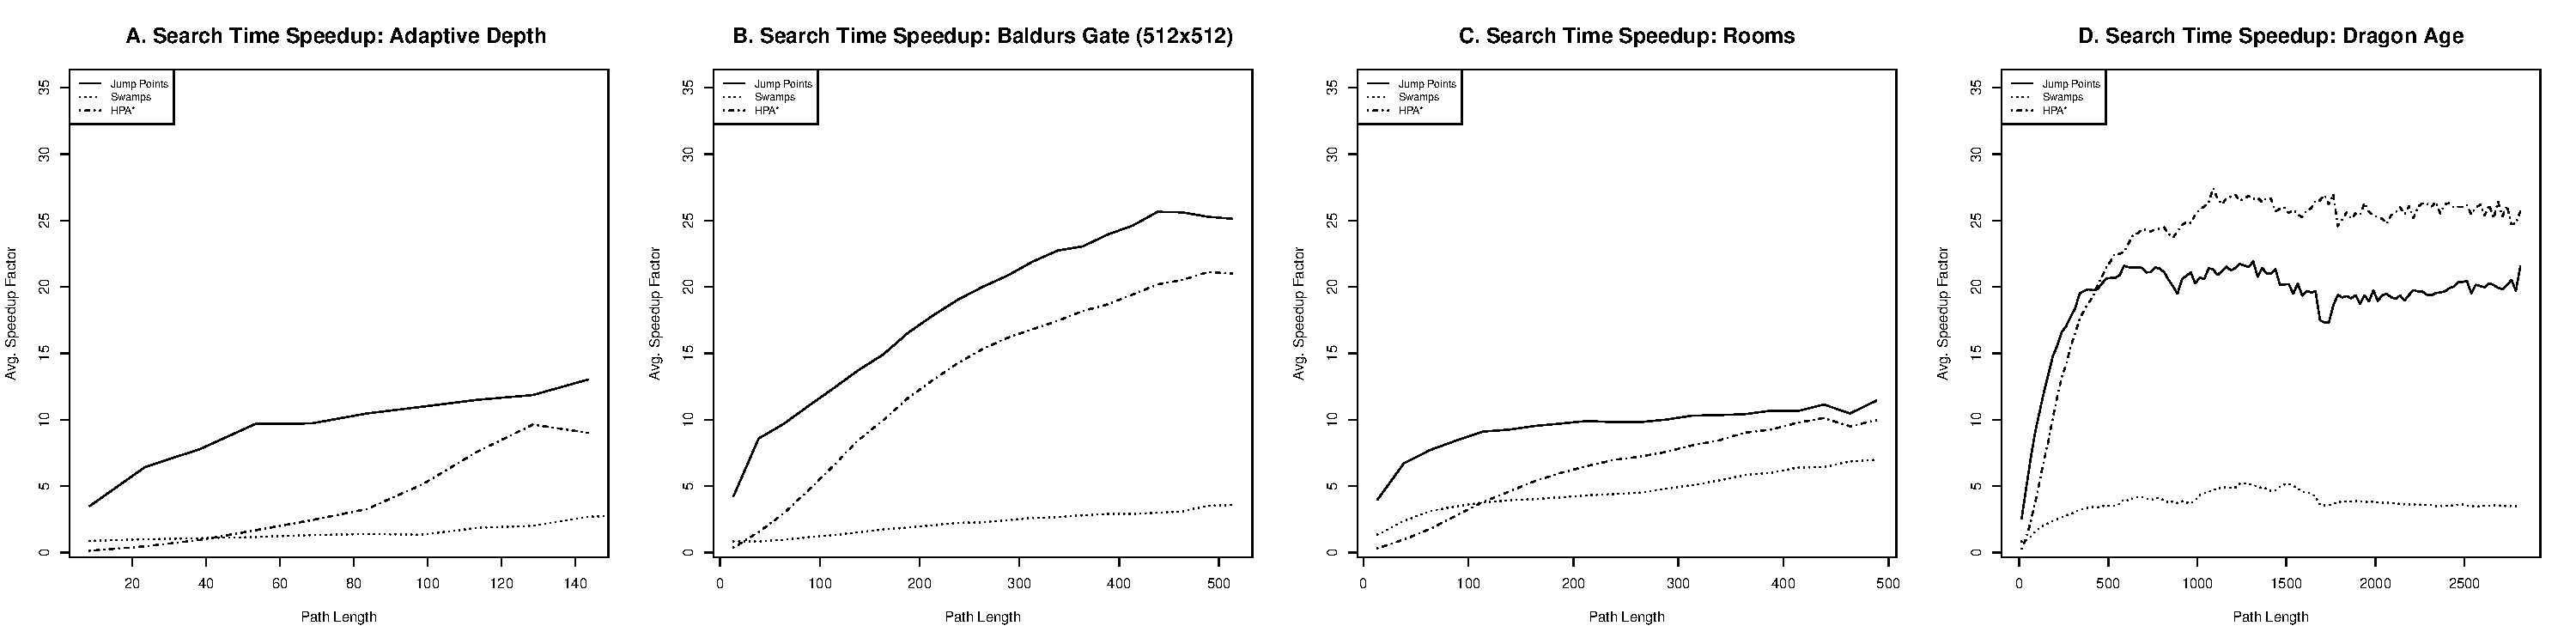
\includegraphics[width=2.0\columnwidth, trim = 10mm 10mm 10mm 0mm]
		{diagrams/speedup.pdf}
   \end{center}
   \caption{Average A* speedup on each of our four benchmarks. 
	Results are given in terms of relative search time improvement.}
\label{fig:speedup}
\end{figure*}

\textbf{Comparison with Swamps: }
We begin by comparing jump points to Swamps\cite{pochter10}: an optimality
preserving pruning techniques for speeding up pathfinding.  When evaluating
Swamps we used the authors' source code, and their implementation of A*, and ran
all experiments using their recommended running parameters: a swamp seed radius
of 6 and ``no change limit'' of 2.

As per Figure \ref{fig:speedup}, jump point pruning shows a convincing search
time improvement over Swamps across all benchmarks.  The largest differences are
observed on Baldur's Gate and Dragon Age where searching with jump points
reaches the goal 20-26 times sooner, on average, while Swamps attains only a 3-5
times speedup.  Similar trends are observed when looking at Table
\ref{table:nodes}, where the improvement to the total number of nodes expanded
is even more pronounced.

Based on these results we conclude that while Swamps are effective for
identifying areas of the map not relevant to reaching the goal, those which
remain still require significant effort to search.  Jump points use a much
stronger yet orthogonal strategy to prove that many nodes in the search space
never require expansion.  As the two ideas are complementary we posit that they
could be easily combined: first, apply a Swamps-based decomposition to prune
areas not relevant to the current search.  Then, use jump points to search the
remaining portions of the map.

\textbf{Comparison with HPA*: }
Next, we compare jump points pruning to the HPA* algorithm~\cite{botea04}.
Though sub-optimal, HPA* is very fast and widely applied in video games. We
compare against it to establish whether or not jump points are equally
applicable in similar contexts.  When evaluating HPA* we used our own
implementation of the algorithm which we configured with a single-level
hierarchy and a fixed cluster size of 10.  These settings are recommended by the
original authors who note that larger cluster sizes and more levels can often
incur significant insertion overhead.

As per Figure \ref{fig:speedup}, jump points pruning is shown to be 
highly competitive with HPA*.
On Adaptive Depth, Baldur's Gate and Rooms jump points are shown to have an 
advantage, improving on HPA* search times by several factors in some cases.
On the Dragon Age benchmark this trend is reversed but the differences are
reasonably small; 22 vs 27 maximum search time speedups.
When looking averge node expansion speedups, in Table \ref{table:nodes} however
we observe that using jump points results in significantly fewer nodes expanded than HPA*.
From this we conclude that jump points and HPA* 
HPA*, the amount of effort required to prune nodes, on some benchmarks, is quite
significant. 

Thus, if optimality is not required, HPA* may be a better choice
in some cases.

Comparing these figures with those for search times provides some indicator 
for the amount of "effort" needed to identify jump point successors for each expanded node.


It is interesting to note that jump point pruning achieves the largest relative
speedup on instances with smaller path lengths
($\leq 100$). Here HPA* search times are dominated by the overhead required to
insert the start and goal into the abstract graph.
As path length increases the advantage provided by jump point pruning is eroded
and, as we see on Dragon Age, HPA* eventually becomes faster.

Jump points and HPA* appear to have complementary strengths.
One direction for further work would be to use jump point pruning to speed up
HPA* insertion times. Furthermore,  jump points could be used to speed up 
HPA* path refinement once an abstract solution is found.
